\chapter{Introducción y Requerimientos de Diseño}
\label{sec:introduccion}

\section{Características de la Señal Electrocardiográfica}

El electrocardiograma (ECG) es el registro de las variaciones de potencial eléctrico generadas por la actividad cardíaca y captadas sobre la piel mediante electrodos de superficie. Desde el punto de vista del procesamiento electrónico de señales, se trata de un biopotencial diferencial de muy baja amplitud y baja frecuencia.

\begin{figure}[!ht]
  \centering
    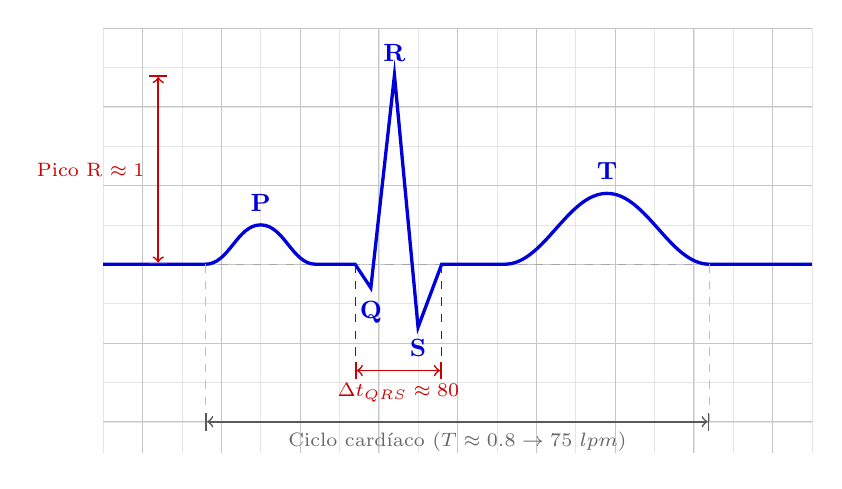
\begin{tikzpicture}[transform shape]
  % Cuadricula en tonos grises acorde a las graficas tecnicas del informe
  \draw[step=0.5, color=gray!20, line width=0.1pt] (-0.5, -2.4) grid (8.5, 3.0);
  \draw[step=1.0, color=gray!45, line width=0.25pt] (-0.5, -2.4) grid (8.5, 3.0);

  % Linea isoelectrica de referencia (0 V)
  \draw[dashed, color=gray!70, line width=0.5pt] (-0.5, 0) -- (8.5, 0);

  % Trazado de la senal de biopotencial ECG en azul (curva principal)
  \draw[color=blue!85!black, very thick, smooth] 
    (-0.5, 0) -- (0.8, 0) 
    .. controls (1.1, 0) and (1.2, 0.5) .. (1.5, 0.5)
    .. controls (1.8, 0.5) and (1.9, 0) .. (2.2, 0)
    -- (2.7, 0)
    -- (2.9, -0.3) % Q
    -- (3.2, 2.4)  % R
    -- (3.5, -0.8) % S
    -- (3.8, 0)    % Punto J
    -- (4.6, 0)
    .. controls (5.1, 0) and (5.4, 0.9) .. (5.9, 0.9)
    .. controls (6.4, 0.9) and (6.7, 0) .. (7.2, 0)
    -- (8.5, 0);

  % Identificacion clara de las ondas P, Q, R, S, T
  \node[above, font=\bfseries\small, color=blue!85!black] at (1.5, 0.55) {P};
  \node[below, font=\bfseries\small, color=blue!85!black] at (2.9, -0.35) {Q};
  \node[above, font=\bfseries\small, color=blue!85!black] at (3.2, 2.45) {R};
  \node[below=1pt, font=\bfseries\small, color=blue!85!black] at (3.5, -0.8) {S};
  \node[above, font=\bfseries\small, color=blue!85!black] at (5.9, 0.95) {T};

  % Cota vertical de amplitud de pico R (en rojo sutil)
  \draw[|<->|, semithick, color=red!80!black] (0.2, 0) -- (0.2, 2.4);
  \node[anchor=east, font=\scriptsize, color=red!80!black] at (0.15, 1.2) {Pico R $\approx \SI{1}{\milli\volt}$};

  % Cota de duracion temporal del complejo QRS (determina frecuencia de corte fH)
  \draw[dashed, color=red!60!black, line width=0.35pt] (2.7, 0) -- (2.7, -1.35);
  \draw[dashed, color=red!60!black, line width=0.35pt] (3.8, 0) -- (3.8, -1.35);
  \draw[|<->|, semithick, color=red!80!black] (2.7, -1.35) -- (3.8, -1.35);
  \node[below=1pt, font=\scriptsize\bfseries, color=red!80!black] at (3.25, -1.35) {$\Delta t_{\text{QRS}} \approx \SI{80}{\milli\second}$};

  % Cota del ciclo cardiaco completo (determina frecuencia fundamental f0)
  \draw[dashed, color=gray!50, line width=0.35pt] (0.8, 0) -- (0.8, -2.0);
  \draw[dashed, color=gray!50, line width=0.35pt] (7.2, 0) -- (7.2, -2.0);
  \draw[|<->|, semithick, color=gray!70!black] (0.8, -2.0) -- (7.2, -2.0)
    node[midway, below, font=\scriptsize, color=gray!80!black] {Ciclo cardíaco ($T \approx \SI{0.8}{\second} \rightarrow 75\ \text{lpm}$)};

\end{tikzpicture}
%
  \caption{Forma de onda un electrocardiograma (ondas P, QRS y T).}
  \label{fig:morfologia_ecg}
\end{figure}

El trazado característico de cada latido normal presenta tres componentes principales (Figura~\ref{fig:morfologia_ecg}):
\begin{itemize}
  \item \textbf{Onda P}: Pequeña deflexión inicial de baja frecuencia y amplitud reducida (típicamente entre $\SI{0.1}{\milli\volt}$ y $\SI{0.3}{\milli\volt}$).
  \item \textbf{Complejo QRS}: Señal de tipo pulsante rápida que concentra la mayor amplitud ($\sim \SI{1}{\milli\volt}$) y las componentes de mayor frecuencia del trazado, con una duración aproximada de $\SI{80}{\milli\second}$ a $\SI{120}{\milli\second}$.
  \item \textbf{Onda T}: Deflexión posterior más suave que marca el fin del ciclo de bombeo.
\end{itemize}

La tensión diferencial se obtiene conectando el electrodo del brazo izquierdo ($V_{\text{LA}}$) a la entrada no inversora y el electrodo del brazo derecho ($V_{\text{RA}}$) a la entrada inversora:
\begin{equation*}
  v_d = V_{\text{LA}} - V_{\text{RA}}
\end{equation*}

Se emplea además un electrodo de referencia conectado a la pierna derecha (RL), el cual se une a la masa analógica del instrumento para fijar el potencial del paciente respecto al circuito de medición.

\section{Desafíos Electrónicos en la Adquisición de la Señal}

El acondicionamiento analógico de biopotenciales presenta cuatro dificultades concretas que condicionan la arquitectura del circuito:
\begin{enumerate}
  \item \textbf{Muy baja amplitud útil}: La señal cardíaca diferencial sobre la piel tiene una amplitud de apenas $\SI{0.5}{\milli\volt\text{pp}}$ a $\SI{2}{\milli\volt\text{pp}}$. Por lo tanto, el circuito requiere una ganancia de tensión de al menos $1000\ \text{V/V}$ ($\SI{60}{\decibel}$) para entregar un nivel normalizado de $\SI{1}{\volt\text{pp}}$, apto para su visualización en osciloscopio o su digitalización mediante un conversor A/D.
  \item \textbf{Interferencia de red a $\SI{50}{\hertz}$}: El cuerpo humano actúa como una antena que capta campos electromagnéticos de la red eléctrica por acoplamiento capacitivo. Esta tensión de modo común puede superar los cientos de milivoltios (mucho mayor que la propia señal cardíaca), por lo que el amplificador debe ofrecer una Relación de Rechazo de Modo Común (RRMC) sumamente elevada ($\gg \SI{80}{\decibel}$) para cancelar dicha interferencia.
  \item \textbf{Tensión continua de contacto electrodo-piel}: El contacto entre el electrodo metálico y la piel con gel conductor genera una tensión galvánica continua de semicelda que puede alcanzar hasta $\pm \SI{300}{\milli\volt}$. Si esta continua se amplificara con la ganancia diferencial total, saturaría inmediatamente los amplificadores contra los rieles de alimentación. Por ello, el circuito debe poseer acoplamiento capacitivo o filtrado pasaaltos con corte en $f_L \approx \SI{0.05}{\hertz} - \SI{0.07}{\hertz}$ para bloquear la continua.
  \item \textbf{Alta impedancia de la piel}: La epidermis presenta una
      impedancia de contacto que suele ubicarse entre $\SI{5}{\kilo\ohm}$ y
        $\SI{100}{\kilo\ohm}$. Para evitar atenuación de la señal por efecto de
        carga resistiva, las entradas del amplificador deben presentar una
        impedancia de entrada muy alta ($Z_i \gg \SI{10}{\mega\ohm}$), lo que
        motiva el uso de amplificadores con transistores de efecto de campo
        (tecnología BiFET/JFET).
\end{enumerate}

\section{Selección del circuito a emplear}

Para dimensionar adecuadamente la solución circuital, conviene analizar por qué las topologías más simples resultan insuficientes para esta aplicación:

\begin{itemize}

  \item \textbf{Amplificador simple no inversor}: Como la interferencia de red a
      $\SI{50}{\hertz}$ captada por el cuerpo puede superar ampliamente la
        magnitud de la señal cardíaca, un amplificador simple referido a masa
        carece de capacidad de rechazo de modo común. Se requiere de forma obligatoria una topología
        diferencial.

  \item \textbf{Restador diferencial clásico de un solo operacional}: Un
      restador convencional presenta impedancias dispares ($R_1$ frente a $R_3 +
        R_4$) comparables a la impedancia piel-electrodo ($\SI{5}{\kilo\ohm}$ a
        $\SI{100}{\kilo\ohm}$). Esto genera atenuación por carga y provoca que
        cualquier desbalance entre electrodos
        rompa la simetría del puente, reduciendo el CMRR a valores inferiores a
        $\SI{40}{\decibel} - \SI{50}{\decibel}$.

  \item \textbf{Amplificador de Instrumentación}:

  \begin{enumerate}

      \item \textit{Impedancia de entrada muy alta en ambos terminales}: Las señales ingresan directamente a los
          terminales no inversores de los buffers $U_1$ y $U_2$.
    \item \textit{Amplificación diferencial selectiva }: La primera etapa entrega una ganancia diferencial elevada
          ($A_{vd1} = 1 + 2R_2/R_1$) mientras que atenúa el modo común.
    \item \textit{Ajuste de ganancia con un único resistor ($R_1$)}: Permite
        modificar o calibrar la amplificación global variando únicamente la
          resistencia central $R_1$, sin comprometer el balance del puente
          restador.
  \end{enumerate}
\end{itemize}

\section{Especificaciones de Diseño}

En función de los requerimientos analizados, el circuito a desarrollar debe cumplir con los parámetros fijados en el Cuadro~\ref{tab:especificaciones}.

\begin{table}[!ht]
  \centering
  \caption{Especificaciones impuestas para el diseño del amplificador de instrumentación.}
  \label{tab:especificaciones}
  \resizebox{\textwidth}{!}{%
  \begin{tabular}{|l|c|l|}
    \hline
    Parámetro & Valor de diseño & Justificación técnica \\ \hline
    Ganancia diferencial ($A_{md}$) & $\SI{60}{\decibel}$ ($1000\ \text{V/V}$) & Escala entrada de $\SI{1}{\milli\volt\text{pp}}$ a salida de $\SI{1}{\volt\text{pp}}$ \\ \hline
    Frecuencia de corte inferior ($f_L$) & $\SI{0.05}{\hertz}$ a $\SI{0.07}{\hertz}$ & Bloquea derivas de continua \\ \hline
    Frecuencia de corte superior ($f_H$) & $\SI{70}{\hertz}$ a $\SI{100}{\hertz}$ & Atenúa ruido muscular (EMG) e interferencias de alta frecuencia \\ \hline
    Rechazo de Modo Común (RRMC) & $\gg \SI{80}{\decibel}$ & Atenúa la interferencia de red de $\SI{50}{\hertz}$ \\ \hline
    Impedancia de entrada ($Z_i$) & $> \SI{5}{\mega\ohm}$ & Evita caída de tensión por impedancia de contacto del electrodo \\ \hline
    Acoplamiento interetapas & Corriente alterna (CA) & Bloquea corrimientos de offset y evita saturación \\ \hline
  \end{tabular}%
  }
\end{table}
